\documentclass[a4paper,12pt]{article}
\usepackage{graphicx}
\usepackage[dvipsnames]{xcolor}
\usepackage{wrapfig}
\usepackage{color}
\usepackage{graphicx}
\usepackage{subfigure}
\usepackage{multirow}
\usepackage[section] {placeins}
\usepackage{tikz}
\usepackage{amsmath}
\usetikzlibrary{matrix,calc}
\usetikzlibrary{positioning}
\usetikzlibrary{matrix}
\pgfdeclarelayer{background}
\pgfsetlayers{background,main}
\usepackage[hidelinks]{hyperref}
\usepackage[nottoc]{tocbibind}

\definecolor{darkred}{rgb}{0,0,0.5}
\definecolor{darkgreen}{rgb}{0,0.5,0}
\definecolor{darkblue}{rgb}{0.5,0,0}
\hypersetup{ colorlinks, linkcolor=darkblue, filecolor=darkgreen, urlcolor=darkred, citecolor=darkblue}

\begin{document}
\begin{titlepage}
\begin{center}
	\textsc{\LARGE Indian Institute of Technology
			\\Bombay} \\[2.5cm]
	\begin{figure}[ht!]
	\begin{center}
		
\includegraphics[scale = 1.4]{images/1}
	\end{center}
	\end{figure}

    \vspace*{-0.6cm}
	\hrule \hrule \hrule
	\vspace{0.5cm}	
	\textsc{\Large CS 492 : BTP Stage I}\\[0.5cm]
	% Title
	{\huge \bfseries Erlang Distributed File System (eDFS)} \\[0.5cm]
	\hrule \hrule \hrule
	\vspace{4cm}
	
	% Author and supervisor
	\begin{minipage}{0.4\textwidth}
	\begin{flushleft} \large
		\emph{By:} \\
		Aman Mangal (100050015)
	\end{flushleft}
	\end{minipage}
	\begin{minipage}{0.4\textwidth}
	\begin{flushright} \large
		\emph{Coordinator:} \\
		Prof. G. Sivakumar
	\end{flushright}
	\end{minipage}
	\vspace{0.5cm}
	
	% Bottom of the page
	{\large \today}
\end{center}
\end{titlepage}
\tableofcontents
\vspace{0.5cm}
\hrule \hrule \hrule
\newpage

\section*{Abstract}
\addcontentsline{toc}{section}{Abstract}
It is extremely difficult for single system to provide high availability, fast response, large data storage and low cost all at the same time. We need multiple systems running in parallel working closely together towards the same goal. We call such systems \textit{Distributed Systems}. Permanent storages are key component to store data and we, therefore, need Distributed File System (DFS). It satisfies the needs of applications that process large volumes of data such as search engines, data mining applications etc.

Erlang \cite{erlang} is recently developed general purpose highly concurrent functional programming language. It was designed to support distributed, fault tolerant, scalable, non-stop applications. It has been used in production systems (e.g. AXD301 ATM switch) with an uptime percentage of 99.9999999\% (nine nine's) \cite[p.~170]{armstrong} \cite{blog_joe}. It is being used by \textbf{Facebook, Github, Riak, Amazon} etc. to develop large distributed systems.

We have leveraged the distributed capabilities of Erlang and have developed yet another DFS namely Erlang Distributed File System (eDFS). We describe the architecture of eDFS in this report. We also look at history of DFSs and compare with eDFS. The main focus has been scalability, efficiency and simplicity while developing the file system. Map reduce has also been implemented for the purpose of testing.

\section{Background}
Distributed File System is an extension of file system which manages files and data on multiple storage devices and provides more performance and reliability using various modern techniques. Outside world only sees it as a single storage device and thus simplifying the interface to a great extent. It also provides location transparency and redundancy to improve data availability in case of failure or heavy load.

Initially DFSs were implemented as part of operating system of each of the connected computers. They either added a software subsystem to UNIX kernel as in Unix United \cite[p.~342]{old_dfs}  or have developed distributed kernel from scratch like Locus \cite[p.~345]{old_dfs}. These DFSs have treated failure as exceptions and focused on sharing of resources. Network File System (NFS) protocol \cite[p.~351]{old_dfs} was developed in this sequence to perform remote file operations.

In recent years, there has been as explosion of interest in computing using clusters of commodity or shared resources. Recently developed the Hadoop Distributed File System \cite{hadoop} and the Google File System \cite{ghemawat03} are designed for use in these commodity computing clusters with a prototypical workload consisting of write once, high throughput, sequential I/O. These systems are cluster based and typically store the metadata separate from the actual data. They provide reliability by replication and consider component failures as norm rather than exceptions.

eDFS is developed with the same strategy using Erlang distributive capabilities. It provides network transparency, location transparency, server and client side caching for high performance, fault tolerance and scalability to some extent. It is highly concurrent and reliable distributed file system. Security issues are not handled as of now, upcoming versions of eDFS may provide security as well.

\section{History of DFS}
\subsection{Unix United \cite[p.~342]{old_dfs}}


\subsection{Locus \cite[p.~345]{old_dfs}}

\subsection{Sun Network File System (Sun NFS) \cite[p.~351]{old_dfs}}

\subsection{Sprite \cite[p.~357]{old_dfs}}

\subsection{Andrew \cite[p.~360]{old_dfs}}

\subsection{Lustre}

\subsection{Panasas}

\subsection{Red Hat Global File System}

\subsection{Haddop Distributed File System (HDFS) \cite{hadoop}}

\subsection{Google File System (GFS) \cite{ghemawat03}}

\subsection{TidyFS \cite{tidyfs}}

\subsection{Green HDFS}

\section{Motivation}

\section{Design Overview}
\subsection{Architecture}
A cluster of eDFS contains a master node, many worker nodes and one or more than one client servers as shown in figure \ref{edfs_design}. Client communicate with client server in order to perform operations on file system. Client can be a browser or any other application which can communicate over tcp/ip connection. Client server can directly communicate to master node or any worker node. Multiple clients can perform operations on file system at the same time using same client server. Multiple client servers can be deployed for load balancing.

All the communication between client and any other node (master or worker) uses standard Bert protocol \cite{bert} unless it is simply message passing in Erlang. Each time a client wants to perform operation on file system, it connects to client server. The client server in turn connects to master node or worker node depending upon the type of request. The client and each worker node creates separate processes corresponding to the operations performed on a single file. Every process has an associated time-out giving fault tolerance to the system.

\begin{figure}[h]
  \begin{center}
    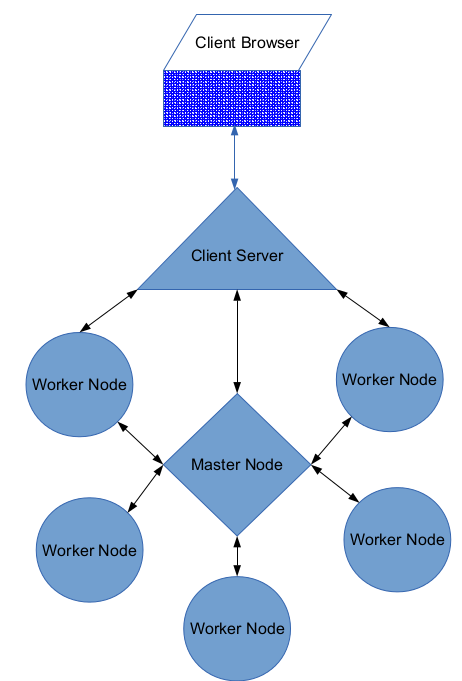
\includegraphics[scale = 0.5]{images/design}
  \end{center}
  \caption{eDFS design}
  \label{edfs_design}
\end{figure}

\subsection{Master node (Metadata Server)}
Master node takes care of handling metadata. It is stored in mnesia in ets tables only. Each file is divided into chunks of approximately equal size. Every chunk is assigned a unique id and stored on multiple worker node based on the replication factor of the file. Following is the table sotred in mnesia-
\begin{table}[h]
\centering
\begin{tabular}{|c|}
\hline 
name \\ 
\hline 
replication factor \\ 
\hline 
chunks \\ 
\hline 
\end{tabular} 
\end{table}

\begin{itemize}
\item \textbf{Name:} name of the file
\item \textbf{Replication Factor:} number of replicas of each chunk
\item \textbf{Chunks:} list of all the chunks of the file stored as \{id, byte begin, byte end, replicas\}
\item \textbf{Id:} chunk id
\item \textbf{Byte begin:} byte number of first byte in the chunk
\item \textbf{Byte end:} byte number of last byte in the chunk
\item \textbf{Replicas:} list of worker ids where replication of the chunk are stored
\end{itemize}

We may support multiple master node and replication of metadata in future.

\subsection{Generation of Chunk Id}
Chunk id is a unique randomly generated string. The chunk is stored with the same name on every worker node. The name can only contain letters a-z, A-Z, 0-9, ".", "\_" (64 letters). It is assumed that name is calculated with less than a million per sec frequency.  Timestamp from operating system is converted into an equivalent representation of a random string and used as the name of a chunk. It is represented using 8 letters (~64 bits). It is possible to generate such ids upto year of 2170 which is approximately 200 years later than the time since when cpu counts the number of seconds (1970).

\subsection{Worker Node}


\section{System Interaction}
\subsection{OTP Hierarchy}
\subsection{Data Flow}
\subsection{Data Replication}
\subsection{Garbage Collection}

\section{Future Work}

\section{Testing}
\subsection{Map Reduce}

\begin{thebibliography}{99}
\bibitem{erlang}
  http://www.erlang.org/

\bibitem{armstrong}
  \textsc{Joe Armstrong},
  "Making Reliable Distributed Systems in the Presence of Software Errors",
  \emph{A Dissertation submitted to the Royal Institute of Technology Stockholm}
  Sweden, December 2003.

\bibitem{blog_joe}
  \textsc{Joe Armstrong},
  "What's All the Fuss About Erlang",
  \emph{http://pragprog.com/articles/erlang},
  2007.

\bibitem{old_dfs}
  \textsc{Eliezer levy, Abraham silberschatz},
  "Distributed File Systems: Concepts and Examples",
  \emph{ACM Computing Surveys, Vol. 22, No. 4},
  December 1990.

\bibitem{hadoop}
  \textsc{Konstantin Shvachko, Hairong Kunag, Sanjay Radia and Robert Chansler},
  "The Hadoop Distributed File System"
  Sunnyvale, California USA

\bibitem{ghemawat03}
  \textsc{Sanjay Ghemawat, Howard Gobioff and Shun-Tak Leung},
  "The Google file system",
  \emph{In SOSP '03: Proceedings of the nineteenth ACM symposium on Operating systems principles}
  New York, NY, USA, 2003.

\bibitem{tidyfs}
  \textsc{Dennis Fetterly, Maya Haridasan, Michael Isard and Swaminathan Sundararaman},
  "TidyFS: A Simple and Small Distributed File System".
  \emph{Microsoft Research Technical Report},
  MSR-TR-20110-24



\bibitem{douceur}
  \textsc{John Douceur, Roger Wattenhofer},
  "Optimizing file availability in a server-less distributed file system"
  \emph{In Proceedings of the 20th Symposium on Reliable Distributed Systems},
  2001.

\bibitem{saito}
  \textsc{Yasushi Saito and Marc Shapiro},
  "Optimistic Replication",
  \emph{ACM Computing Surveys, Vol. 37, No. 1},
  March 2005, pp. 42-81.

\bibitem{satya}
  \textsc{Satyanarayanan, M.},
  "A Survey of Distributed File Systems",
  \emph{Technical Report CMU-CS-89- 116, Department of Computer Science, Camegie Mellon University},
  1989.

\bibitem{nelson}
  \textsc{Nelson, M.N., et al},
  "Caching in the Sprite Network File System",
  \emph{ACM Transactions on Computer Systems},
  February, 1988.

\bibitem{rowe}
  \textsc{Rowe, L.A., Birman, K.P.},
  "A Local Network Based on the Unix Operating System",
  \emph{IEEE Transactions on Software Engineering SE-8(2)},
  March, 1982.

\bibitem{edmund}
  \textsc{Edmund B. Nightingale, Peter M. Chen, and Jason
Flinn},
  "Speculative Execution in a Distributed File System",
  \emph{ACM SOSP’05},
  October 23–26, 2005, Brighton, United Kingdom.

\bibitem{howard}
  \textsc{Howard J. H., Kazar M. L., Menees S. G., Nichols D. A.,
Satyanarayanan M., Sidebotham R. N. and West M. J.}
  "Scale and performance in a distributed file system",
  \emph{ACM Transactions on Computer Systems, Vol. 6, Issue1},
  February 1988

\bibitem{panasas}
  \textsc{Nagle D., Serenyi D., Matthews A.},
  "The Panasas ActiveScale Storage Cluster: Delivering Scalable High Bandwidth Storage",
  \emph{Proceedings of the 2004 ACM/IEEE conference on Supercomputing, pp. 53-},
  2004.

\bibitem{yu}
  \textsc{Yu W., Liang Sh., Panda D.K.},
  "High Performance Support of Parallel Virtual File System (PVFS2) over Quadrics",
  \emph{Proceedings of the 19th annual international conference on Supercomputing, pp. 323-331},
  2005.

\bibitem{chandramohan}
  \textsc{Chandramohan A. Thekkath, et al},
  "Frangipani: A Scalable Distributed File System",
  \emph{System Research Center, Digital Equipment Corporation},
  Palo Alto, CA, 1997.

\bibitem{liskov}
  \textsc{Barbara Liskov, et al},
  "Replication in the Harp File System",
  \emph{Laboratory of Computer Science, MIT, Cambridge},
  CA, 1991.
\end{thebibliography}

\end{document}
